\documentclass[12pt, openright,oneside, a4paper, english, brazil, section = TITLE, ubsection = Title]{article}

% ----------------------------
% Pacotes básicos 
% ----------------------------
% Referências
\usepackage[brazilian,hyperpageref]{}	
\usepackage{hyperref}
\usepackage[alf]{abntex2cite}			

% Fonte e codificação (acentuação)
\usepackage{lmodern}       
\renewcommand{\sfdefault}{ppl}
\usepackage[T1]{fontenc}	
\usepackage[utf8]{inputenc}	
% Tabelas e Figuras
\usepackage{ctable}             
\usepackage{multirow}
\usepackage{array}
\usepackage{float}              
\usepackage{longtable}          
\usepackage{xcolor,colortbl}    
\usepackage{booktabs}           
\usepackage{graphicx}			
\usepackage{subfig}             
\usepackage{caption}            
\usepackage{epstopdf}           

% Equações e símbolos
\usepackage{amsmath}            
\usepackage{nomencl} 
\usepackage{cleveref} 
\usepackage{calrsfs}
\usepackage{amssymb}
\usepackage{psfrag}
\usepackage[brazil]{babel}
% Texto
%\usepackage[showframe,heightrounded]{geometry}
\usepackage{geometry}
\usepackage{indentfirst}		
\usepackage{color}				
\usepackage{microtype} 			
\usepackage{lastpage}			
\usepackage{enumitem}                % Para os itens em letras
\usepackage{lipsum}
\usepackage{lastpage}
\usepackage{tablefootnote}
\usepackage{pdflscape}
\usepackage{scalefnt}
\usepackage[stable]{footmisc}
\usepackage{cases}
% ----------------------------------------------------------
% Configurações do texto
% ----------------------------------------------------------

% Recuo do parágrafo :
\setlength{\parindent}{1.5cm}
\setlength{\parskip}{0cm} 
\geometry{a4paper}%,left=3cm,right=2cm,top=3cm,bottom=2cm} % SEMPRE BOM VER A DOCUMENTAÇÃO
\hoffset = -1in
\voffset = -1in
\oddsidemargin = 1.5cm
\topmargin = 2cm
\headheight = 0pt
\headsep = 6pt % multiplicar por 0.03515 para obter cm
\textheight = 249mm
\textwidth = 18cm
\marginparsep = 0pt
\marginparwidth = 0pt
\footskip = 6mm
%
%
%
\usepackage{array}
\newcolumntype{L}[1]{>{\raggedright\let\newline\\\arraybackslash\hspace{0pt}}m{#1}}
\newcolumntype{C}[1]{>{\centering\let\newline\\\arraybackslash\hspace{0pt}}m{#1}}
\newcolumntype{R}[1]{>{\raggedleft\let\newline\\\arraybackslash\hspace{0pt}}m{#1}}
%
%
%
\newtheorem{teorema}{Teorema}[section]
\newtheorem{propriedade}[teorema]{Condição}
\newtheorem{lema}[teorema]{Lema}
\newtheorem{corolario}[teorema]{Corolário}
\newtheorem{proposicao}[teorema]{Proposição}
\newtheorem{definicao}[teorema]{Definição}
\newtheorem{exemplo}[teorema]{Exemplo}
\newtheorem{af}[teorema]{AF}
\newtheorem{exercicio}[teorema]{Exercício}
\newtheorem{algoritmo}{Algoritmo}[section]
\newtheorem{exc}{}[section]
\newtheorem{impl}{}[section]
\newtheorem{hip}{H\hspace{-.12cm}}
\newtheorem{res}{R\hspace{-.12cm}}
%
%
%
\newcommand{\rel}{\Bbb R^{\ell}}
\newcommand{\rell}{\mathbb R^{\ell}_{+}}
\newcommand{\rr}{\mathbb R}
\newcommand{\bb}[1]{\boldsymbol{#1}}
\newcommand{\ol}[1]{\overline{#1}}
\newcommand{\hess}{\nabla^2(f(\bb{x}))}

\newcommand{\kktmax}[3]{
\begin{aligned}
& \underset{#1}{\text{maximizar}}
& & {#2} \\
& \text{sujeito a} 
& & {#3} \\
\end{aligned}}

\newcommand{\kktmin}[3]{
\begin{aligned}
& \underset{#1}{\text{minimizar}}
& & {#2} \\
& \text{sujeito a} 
& & {#3} \\
\end{aligned}}

%  Novos macros
\newcommand{\R}{\mathbb{R}}
\newcommand{\N}{\mathbb{N}}
\newcommand{\U}{\mathcal{U}}
\newcommand{\Rn}{{\R}^n}
\newcommand{\sumin}{\sum_{i=1}^n}
\newcommand{\Rl}{{\R}^\ell}
\newcommand{\Rm}{{\R}^m}
\newcommand{\ind}{1,\ldots,n}
%
%
%
%
%

\title{Uma avaliação da validade da Lei de Okun para o Brasil no período 2013-2019}
\author{Pedro Milreu Cunha \thanks{Mestrando - PPGE/UFPB} \and 
Rony Ramos Cavalcanti da Silva \thanks{Mestrando - PPGE/UFPB} \and 
Valber Gregory Barbosa Costa Bezerra Santos \thanks{Doutorando - PPGE/UFPB}}

\date{}
%
%
%
%
%
%
%
%
%
\begin{document}
\topmargin = 0.2cm
\maketitle

\setlength{\parindent}{0cm}



\textbf{RESUMO} 

O presente estudo objetivou estimar, analisar e verificar a validade da Lei de Okun para a economia brasileira, adaptando o modelo apresentado em \citeonline{Ball2012}. Utilizaram-se dados de emprego, taxa de desemprego e o Produto Interno Bruto (PIB) a preços de mercado decompostos em séries trimestrais de 2013 a 2019.  A estimação fez uso da suavização dos dados temporais por meio do filtro de Hodrick-Prescott (1997), ou filtro HP, técnica cuja validade foi discutida no trabalho \cite{Hodrick1997}; foi feita também uma análise com a aplicação da modelagem \textit{Seemingly Unrelated Regressions} (SUR), juntamente com análise de possíveis quebras estruturais pelo teste de Chow e pelo critério do menor \textit{Bayesian Information Criteria} (BIC). Ao final, verificou-se que a relação de curto prazo negativa entre a taxa de desemprego e produto, apresentada inicialmente \citeonline{Okun1962}, é estável para o Brasil. Além disso, foram obtidos bons ajustes da Lei de Okun em duas especificações distintas, ao menos para o período em consideração.

\textbf{Palavras-chave}: Lei de Okun. Quebra estrutural. Brasil.

\textbf{JEL:}  E01. E24.

\vspace{0.6cm}

\textbf{ABSTRACT} 

The present study aims to estimate, analyze and verify the validity of Okun's Law for the Brazilian economy, adapting the model presented in \citeonline{Ball2012}. Data on employment, unemployment rate and the Gross Domestic Product (GDP) at market prices broken down into quarterly series from 2013 to 2019 are used. The estimation uses the smoothing of temporal data through the Hodrick-Prescott (HP) filter, which has its validity discussed in the paper \cite{Hodrick1997}; an estimation with the application of modeling \textit{Seemingly Unrelated Regressions} (SUR) was also done, together with an analysis of possible structural breaks using both the Chow test and the criterion of the smallest \textit{Bayesian Information Criteria} (BIC). The results show that for the negative short-term relationship between unemployment rate and output, proposed by \citeonline{Okun1962}, is stable for Brazil. Furthermore, it can also be seen that the Brazilian economy adjusted well to two distinct model specifications, at least for the period under consideration.

\textbf{Keywords}: Okun's Law. Structural break. Brazil.

\textbf{JEL:} E01. E24.

\newpage
\topmargin = 2cm
\setlength{\parindent}{1.5cm}

\section{Introdução}

A relação empírica e regular de curto prazo negativa entre a taxa de desemprego e produto é estudada pelo menos desde a contribuição de \citeonline{Okun1962}. Por outro lado, múltiplas evidências demonstram que a taxa natural de desemprego varia durante o tempo com uma grande amplitude \cite{Hall2003}. Desde a crise financeira de 2007, cresce na academia e nos governos o interesse por estudar mais de perto as relações entre força de trabalho e produto, composição dos trabalhadores de uma nação e como as tendências vem se alterando com o passar do anos \cite{Krueger2017}. 

Verifica-se que é nesse cenário que surgem trabalho buscando analisar a estabilidade, forma, tempo e composição das variáveis que integram a "Lei de Okun" em diversos países do mundo, como em \citeonline{Ball2012}, que investigaram a relação de Okun para os Estados Unidos e outros 20 países com economias avançadas. Os autores encontraram, ao final, que para a economia americana, com dados de 1948 a 2013, a relação mostrou-se estável e significativa, implicando que o coeficiente de Okun mantém-se constante no tempo, sendo, no caso, uma boa aproximação da realidade.

Há trabalhos que suscitam métodos e formas aplicáveis a diferentes países, ou grupos de países, que comumente mantém a similaridade ou proximidade de algumas características regionais ou macroeconômicas. \citeonline{Lim2019} estudaram os dados dos Estados Unidos entre 1990 e 2017;\citeonline{Huang2013} utilizaram dados em \textit{cross-section} de países da Organização para a Cooperação e Desenvolvimento Econômico (OCDE) e dos Estados Unidos e também entre estados federados norte-americanos; \citeonline{Zanin2014} analisou os países da OCDE e subclassificou o mercado de trabalho por gênero e por idade para entender a dinâmica de cada faixa-etária. 

Em relação a outros países fora do eixo Estados Unidos e OCDE, \citeonline{Pizzo2019} apresentou um estudo com revisão dos artigos que trataram de alguns países que compõem a América Latina e o Caribe; \citeonline{Kurosaka2014} realizou estudo para avaliação e adequação da Lei de Okun para o Japão, com dados de 1981 a 2010; \citeonline{Marinkov2007} estudaram os dados sul-africanos entre 1970 e 2005. Finalmente, \citeonline{Karim2016} realizaram uma revisão de literatura com autores que estudaram a estabilidade da relação entre desemprego e produto em alguns países da África.

Assim, o presente trabalho teve como objetivo verificar aplicação e estabilidade desta relação ao Brasil, utilizando-se de dados trimestrais de 2013 a 2019, adaptando o modelo apresentado por \citeonline{Ball2012}, tendo como variáveis o emprego, taxa de desemprego e o Produto Interno Bruto (PIB) a preços de mercado. 

Estimou-se o modelo com a utilização da suavização dos dados temporais por meio do filtro de Hodrick-Prescott (HP) \cite{Hodrick1997}. Além disso, foi realizada também uma estimação conjunta de sistema feita com a técnica de \textit{Seemingly Unrelated Regressions} (SUR). Por fim, foi realizada uma análise de possíveis quebras estruturais na equação estimada da Lei de Okun para o Brasil pelo teste de Chow e pelo critério do menor \textit{Bayesian Information Criteria} (BIC).

O presente estudo é dividido em 4 seções, afora a introdução. Na primeira seção, faz-se uma revisão de literatura, em que se procura explorar estudos que, mesmo tendo aplicado diferentes métodos, procuraram verificar a validade e a magnitude dos coeficientes que compõem a relação descrita na Lei de Okun, realizando, também, uma breve explanação da especificação utilizada no presente trabalho sobre a citada relação. Na segunda seção, discorre-se sobre a estratégia empírica, fornecendo informações acerca da origem e organização dos dados utilizados, pormenorizando-se explicitações acerca da forma de estimar a relação de Okun, sobre o filtro HP, SUR e sobre o uso de testes para verificar existência de quebra estrutura. Na terceira parte são apresentados os resultados obtidos com as estimações, bem como tenta-se descrever o porquê dos valores encontrados. Na última seção, realizam-se as considerações finais, concluindo o trabalho.

\section{Revisão de Literatura}

\subsection{Uma revisão da Lei de Okun}

\citeonline{Okun1962} foi quem primeiro debruçou sobre uma possível relação inversa entre produto e taxa de desemprego. Ao testar empiricamente essa hipótese para os Estados Unidos, encontrou uma relação sólida, estimando que a redução de $1\%$ no desemprego se dava mediante ao aumento de $3\%$ do produto. Desde então, diversos trabalho vem investigando não só se a relação é forte e significativa, mas também se é estável ao longo do tempo. 

Assume-se que mudanças na demanda agregada fazem o produto flutuar ao redor do seu valor potencial. Essas mudanças no produto causam a contratação e demissão de trabalhadores pelas firmas, alterando o emprego; variações no emprego movem o desemprego no sentido oposto. Essas relações podem ser vistas no sistema de equações a seguir:

\begin{numcases}{}
E_t - E_t^*= \gamma \cdot (Y_t - Y_t^*) + \eta_t, \quad \gamma > 0 \\ 
U_t - U_t^* = \delta \cdot (E_t - E_t^*) + \mu_t, \quad \delta < 0 \\
U_t - U_t^* = \beta \cdot (Y_t - Y_t^*) + \epsilon_t, \quad \beta < 0 
\end{numcases}
onde $\beta = \delta \cdot \gamma$ e $\epsilon_t = \mu_t + \delta \cdot \eta_t$. Além disso, $E_t$ e $Y_t$ são o logaritmo do produto e do emprego, respectivamente, $U_t$ é a taxa de desemprego e $^*$ indica níveis de longo-prazo. Em especial, \citeonline{Okun1962} estava interessado na equação $(3)$, ou seja, na relação entre o hiato do desemprego e o hiato do produto.

\subsection{A aplicação da Lei de Okun para diferentes países}

\citeonline{Ball2012} testaram a validade e a estabilidade da Lei de Okun para a economia americana entre 1948 e 2011, bem como para 20 economias avançadas, a partir de 1980 até 2011. Os resultados mostraram que a Lei de Okun se manteve estável e que as hipóteses de recuperação sem emprego ou invalidade da lei em face a grande crise de 2008, não se mostram pertinentes ante os dados. 

Para os EUA, os coeficientes estimados giravam em torno de $-0,4$. O trabalho também apontou para a discrepância entre os coeficientes estimados para os diversos países. Para o Japão, o coeficiente foi de $-0,15$, enquanto que para Espanha foi de $-0,85$. Essas divergências podem ser explicadas, em parte, pelas idiossincrasias de cada mercado de trabalho; como apontam os autores, o Japão tem tradição em empregos estáveis, enquanto na Espanha prevalecem contratos temporários. 

\section{Dados e metodologia}

\subsection{Fonte de dados e estatísticas descritivas}

A base de dados utilizada na elaboração do presente artigo foi obtida no site do Ipeadata, na seção de dados macroeconômicos. A tabela abaixo apresenta a descrição das variáveis utilizada, bem como as transformações que foram realizadas nelas: 

\begin{table}[H]
\centering
\caption{Descrição das  variáveis}
\label{tab:dados}
\resizebox{\textwidth}{!}{%
\begin{tabularx}{\textwidth}{lcX} \\
Variável & Nome & Descrição \\ \midrule
$E_t$ & Emprego & $100 \times \ln(\text{pessoas ocupadas [em milhares]})$ \\ \midrule
$U_t$ & Taxa de desemprego & $\%$ da força de trabalho desempregada que está ativamente procurando por um emprego \\ \midrule 
$Y_t$ & Produto & $100 \times \ln(\text{PIB [em milhões]})$ \\ \bottomrule \\
& Fonte: & Ipeadata - Instituto de Pesquisa Econômica Aplicada (IPEA)
\end{tabularx}
}
\end{table}

Para além disso, foi feita a conversão das séries de emprego e desemprego, que antes eram mensais, para a periodicidade trimestral, visando adequar todas as três séries à uma só frequência.\footnote{Para fazer esse processo foi utilizado o comando \textit{aggregate} do pacote \textit{stats}, disponível no R$^{\text{\textregistered}}$ \cite{R2020}.}

\begin{table}[H]
\centering
\caption{Estatísticas descritivas}
\label{tab:estatisticas_descritivas}
\resizebox{\textwidth}{!}{%
\begin{tabular}{lccccccc}
\toprule
Estatística & \multicolumn{1}{c}{N} & \multicolumn{1}{c}{Média} & \multicolumn{1}{c}{Desv. pad.} & \multicolumn{1}{c}{Mín} & \multicolumn{1}{c}{$\mathcal{P}_{25}$} & \multicolumn{1}{c}{$\mathcal{P}_{75}$} & \multicolumn{1}{c}{Máx} \\ \midrule
Taxa de desemprego & 28 & 10,068 & 2,459 & 6,467 & 7,542 & 12,142 & 13,300 \\
Produto & 28 & 1424,882 & 10,802 & 1401,640 & 1417,591 & 1434,147 & 1444,136 \\
Emprego & 28 & 1142,081 & 1,421 & 1139.645 & 1141,294 & 1142,780 & 1145,467 \\ \bottomrule
\end{tabular}%
}
\caption*{\\ Fonte: Elaboração própria baseada nos dados disponíveis em \cite{IPEA2020}.}
\end{table}

Dadas as transformações que foram realizadas, as estatísticas descritivas não informam muita coisa. Considerando apenas a variável que captura o desemprego, uma vez que ela não foi alterada, tem-se que no período de 2013-2019 o Brasil apresentou um valor médio de $10,068\%$ para a taxa de desemprego, enquanto os valores mínimos e máximos foram, respectivamente, de $6,467\%$ e $13,300\%$. Vê-se, portanto, que a série teve uma grande amplitude e também uma variabilidade relativamente elevada, dada aqui pelo valor do desvio-padrão, de $2,459$. 

Na próxima subseção é feita a discussão acerca de como realizar a estimação da Lei de Okun de forma correta.

\subsection{Como estimar a Lei de Okun?}

A primeira opção é estimar a equação $(3)$ diretamente. O problema se encontra em estimar os termos não-observáveis $U_t^*$ e $Y_t^*$. Para contornar isso, pode-se fazer uso do filtro \textit{Hodrick Prescott} (HP), que é discutido na próxima subseção.

A segunda opção é estimar a versão em primeiras diferenças da Lei de Okun, dada pela equação a seguir:
    \begin{equation}
    \Delta U_t = \alpha + \beta \cdot \Delta Y_t + \omega_t
    \end{equation}
onde $\Delta$ é a mudança em relação ao período anterior. Essa equação segue de $(3)$ se assumirmos que $U^*$ é constante e que $Y^*$ cresce a uma taxa constante ($\Delta Y^*$). Fazendo isso, obtemos a equação $(4)$ com $\alpha = -\beta \cdot \Delta Y^*$ e $\omega_t = \Delta \epsilon_t$.

Uma outra opção, no interesse de estimar as relações econômicas derivadas do sistema composto pelas equações $(1), (2)$ e $(3)$ conjuntamente, é fazer uso do modelo de regressões aparentemente não-relacionadas (SUR), discutido mais a frente.

\subsection{Filtro Hodrick-Prescott}

Utilizado amplamente na análise de séries temporais, o filtro HP foi apresentado por \citeonline{Hodrick1997} e tem como ideia básica a \textbf{decomposição de uma série temporal}. Deixe $\{h_t\}_{t=1}^{T}$, denotar o logaritmo de uma variável de uma série temporal. Pode-se decompor $h_t$ em um componente de tendência, $\tau_t$; um componente cíclico, $\pi_t$; e um componente de erro, $\epsilon_t$, de modo que 
\begin{equation}
h_t = \tau_t + \pi_t + \epsilon_t
\end{equation}

Considerando um parâmetro de ponderação, $\lambda > 0$, escolhido de forma ótima, existe um componente de tendência $\tau_t^*$ que satisfaz o seguinte problema:
\begin{equation}
\underset{\tau_t^*}{\operatorname{min}} \left( \sum_{t=1}^T (h_t-\tau_t^*)^2 + \lambda \cdot \sum_{t=2}^{T-1} [(\tau_{t+1}^*-\tau_t^*) - (\tau_t^* - \tau_{t-1}^*)]^2 \right)
\end{equation}

O primeiro termo representa a soma dos quadrados dos desvios, $d_t = h_t - \tau_t^*$, que penaliza o componente cíclico. O segundo termo é uma ponderação da soma dos quadrados das segundas diferenças do componente de tendência. Esse termo penaliza variações na taxa de crescimento do componente de tendência. Quanto maior o valor de $\lambda$, mais suave é a série temporal que resulta do problema de minimização acima. Para um $\lambda$ suficientemente grande, a diferença entre os pares $\tau_{t+1}$ e $\tau_t$ deve ficar arbitrariamente próxima de uma constante $\beta$, de modo que $\tau_t$ se encontre arbitrariamente próximo de $\tau_0 + \beta \cdot t$. Isso implica que conforme $\lambda \to \infty$, o limite das soluções do programa é o ajuste de mínimos quadrados de um modelo de tendência linear.

Naturalmente, o filtro não é unanimidade na comunidade acadêmica, sofrendo diversas críticas, em particular sobre seus problemas de viés relacionados ao final de amostras. Um artigo mais recente e com críticas bem contudentes é \citeonline{Hamilton2018}, intitulado "Why you should never use the Hodrick-Prescott filter", material que os leitores interessados são convidados a consultar. Apesar disso, uma vez que a técnica ainda é utilizada com frequência e com bons resultados, como por exemplo no trabalho de \citeonline{Ball2012}, optou-se por fazer uso da mesma não obstante os seus possíveis problemas.

\subsection{\textit{Seemingly Unrelated Regressions} (SUR)}

Este método apresentado por \citeonline{Zellner1962} é uma generalização do modelo de regressão linear, sendo composto por várias equações de regressões, cada uma com suas respectivas variáveis dependentes e conjuntos potencialmente diferentes de variáveis explicativas.

\begin{numcases}{}
E_t - E_t^*= \gamma \cdot (Y_t - Y_t^*) + \eta_t, \quad \gamma > 0 \\ 
U_t - U_t^* = \delta \cdot (E_t - E_t^*) + \mu_t, \quad \delta < 0 \\
U_t - U_t^* = \beta \cdot (Y_t - Y_t^*) + \epsilon_t, \quad \beta < 0 
\end{numcases}

Cada equação do sistema acima pode ser estimada separadamente utilizando Mínimos Quadrados Ordinários, obtendo resultados que são consistentes. Entretanto, no caso em que os termos de erros das equações são correlacionados, tem-se um ganho de eficiência (pelo menos assintóticamente) ao estimar as equações conjuntamente, fazendo uso, por exemplo, do método dos Mínimos Quadrados Generalizados Factíveis (MQGF).

Em particular, o autor argumenta que "o ganho em eficiência pode ser bastante grande se as variáveis "independentes" em cada equação apresentarem baixa correlação entre si, enquanto os termos de erros forem altamente correlacionadas"\, \cite[p.~3, tradução nossa]{Zellner1962}.

\subsection{Quebra estrutural - teste de Chow e critério do menor \textit{Bayesian Information Criteria} (BIC)}

Para cada potencial ponto de quebra estrutural da série em um intervalo de tempo especificado, uma estatística F é calculada (estatística do teste de Chow)\footnote{
A discussão feita aqui se baseia no manual do pacote \textit{strucchange} (\citeonline{Zeileis2006}), disponível no software R$^\text{\textregistered}$ \cite{R2020}. }. À partir disso, um modelo OLS é estimado para as observações de antes e depois do ponto de mudança e a soma dos quadrados dos resíduos é calculada (ESS). Um outro modelo é estimado para todas as observações, gerando uma soma de quadrados restritas (RSS). Se $n$ é o número de obervações e $k$ é o número de regressores no modelo, então tem-se a seguinte estatística:
\begin{equation} \scriptsize
F = \frac{RSS - ESS}{ESS \cdot (n - 2k)}
\end{equation}
que segue uma distribuição assintótica qui-quadrada com $k$ graus de liberdade e, sob a hipótese de normalidade, $\frac{F}{k}$ tem uma distribuição F exata com $k$ e $n-2k$ graus de liberdade.

A ideia do critério BIC é semelhante, porém em vez de comparar os valores da estatística de Chow com os críticos da distribuição F, é escolhido o número de quebras que gera o menor valor para o BIC, que é usualmente definido da seguinte maneira:
\begin{equation}
\text{BIC} = k \cdot \ln(n) - 2\ln(\hat{L})
\end{equation}
onde $k$ é o número de parâmetros estimados pelo modelo; $n$ é o número de observações e $\hat{L}$ é o valor maximizado da função de verossimilhança do modelo.

Na próxima seção são apresentados os principais resultados do trabalho e suas respectivas discussões.

\section{Resultados}

\subsection{Decomposições}

Nas três figuras a seguir são apresentados, de forma gráfica, os resultados das decomposições das séries históricas do desemprego, emprego e do produto, obtidas utilizando o filtro HP, já discutido anteriormente. É importante destacar que nos gráficos do lado esquerdo, a linha vermelha representa a tendência de longo-prazo, enquanto a linha azul são os próprios valores observados. Nos gráficos do lado direito, tem-se representada a diferença entre os valores observados e a tendência de longo-prazo, ou seja, os hiatos necessários para a estimação da Lei de Okun.

\begin{figure}[H]
	\centering
	\caption{Decomposição - Série trimestral do desemprego - 2013/1:2019/4}
	\label{fig:decomposição_desemprego}
	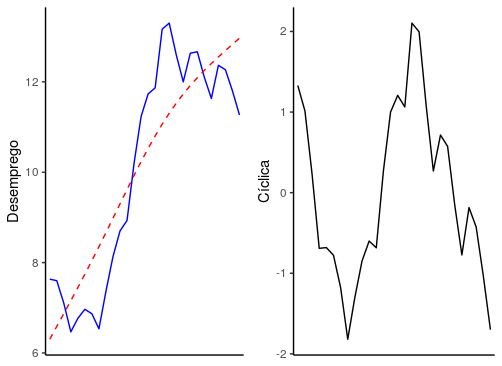
\includegraphics[width=0.45\linewidth]{"Figuras/decomposição_desemprego.png"} \\
\caption*{Fonte: Elaboração própria à partir dos dados disponíveis em \cite{IPEA2020}.}
\end{figure}

\begin{figure}[H]
	\centering
	\caption{Decomposição - Série trimestral do emprego - 2013/1:2019/4}
	\label{fig:decomposição_emprego}
	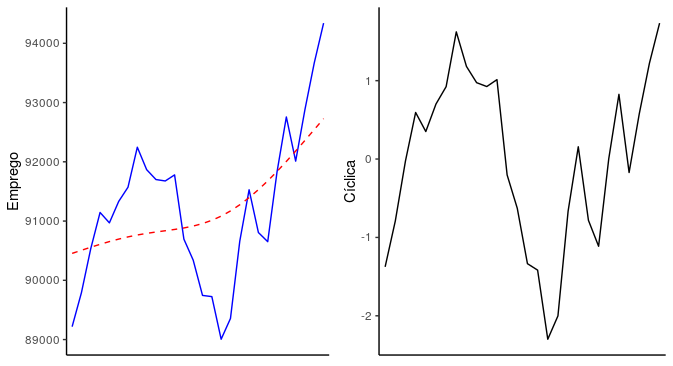
\includegraphics[width=0.45\linewidth]{"Figuras/decomposição_emprego.png"} \\
\caption*{Fonte: Elaboração própria à partir dos dados disponíveis em \cite{IPEA2020}.}
\end{figure}

\begin{figure}[H]
	\centering
	\caption{Decomposição - Série trimestral do produto - 2013/1:2019/4}
	\label{fig:decomposição_PIB}
	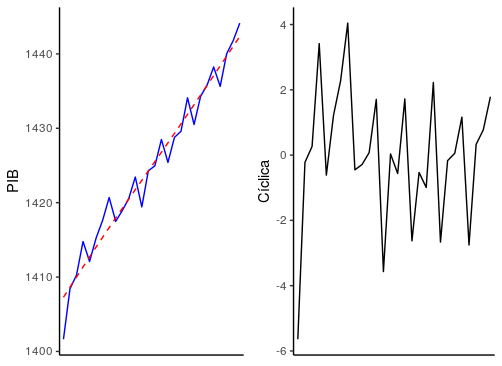
\includegraphics[width=0.45\linewidth]{"Figuras/decomposição_produto.png"} \\
\caption*{Fonte: Elaboração própria à partir dos dados disponíveis em \cite{IPEA2020}.}
\end{figure}

De forma geral, vê-se que a série com a maior quantidade de flutuações ao redor de seu valor de longo-prazo foi a do produto, enquanto que as séries de desemprego e emprego apresentaram períodos mais longos nos quais se encontram acima ou abaixo de seus valores potenciais. Na subseção a seguir são apresentados e discutidos os resultados.

\subsection{Estimações}

A Lei de Okun apresentou um excelente ajuste aos dados da economia brasileira, sendo obtido um $R^2$ ajustado de $0,490$ no modelo com o melhor ajuste para a equação estimada em níveis.\footnote{Conforme obtido em \citeonline{Ball2012}, para o presente trabalho a inclusão de dois \textit{lags} das variáveis independentes nas equações estimadas contribuiu para a melhora dos ajustes dos modelos.} Na tabela a seguir são apresentados os resultados da estimação para $\lambda = 1600$ e $\lambda = 16000$. Uma vez que o melhor ajuste obtido foi para $\lambda = 1600$, as análises seram feitas baseadas nessa estimação.

O coeficiente o hiato do produto foi significativo à $1\%$, apresentando também uma magnitude bastante expressiva. Isso indica que um aumento de $1\%$ no hiato do produto reduz o hiato do desemprego em $0,332\%$, resultado semelhante aquele obtido em \citeonline{Gouveia2015} para a economia brasileira no período 1996-2013. Além disso, nota-se claramente que há um efeito defasado do produto sobre o desemprego, que é capturado pelo dois \textit{lags} utilizados, sendo ambos estatisticamente significativos e com coeficientes de elevada magnitude. Isso aponta que as mudanças no hiato do produto não geram apenas um efeito contemporâneo, sendo necessário mais tempo para que todos os impactos sejam sentidos no hiato do desemprego.

\begin{table}[H]
\centering
\caption{Estimativas da Lei de Okun (dados trimestrais, 2013/1-2019/4) \\
\quad Equação estimada em níveis: $U_t - U_t^* = \mathcal{L}[0,1,2]\{\beta \cdot (Y_t - Y_t^*)\}  + \epsilon_t$}
\label{tab:okun_nivel}
\begin{tabular}{lc} \\ \toprule
Filtro HP $\lambda = 1600$ &  \\
Hiato do produto & $-0,332^{***}$ \\
 & $(0,074)$ \\
$\mathcal{L}[1]$ (Hiato do produto) & $-0,288^{***}$ \\ & $(0,062)$  \\ 
$\mathcal{L}[2]$ (Hiato do produto) & $-0,111^{**}$ \\ & $(0,049)$ \\
Obs. & $26$ \\
$R^2$ ajustado & $0,490$ \\
RSE & $0,747$ (df = $23$) \\ F & $9,310^{***}$ (df = $3;23$) \\ \midrule
Filtro HP $\lambda = 16000$ &  \\
Hiato do produto & $-0,371^{***}$ \\
 & $(0,088)$ \\
$\mathcal{L}[1]$ (Hiato do produto) & $-0,306^{***}$  \\ & $(0,076)$  \\ 
$\mathcal{L}[2]$ (Hiato do produto) & $-0,095$ \\ & $(0,061)$  \\
Obs. & $26$ \\
$R^2$ ajustado & $0,442$ \\
RSE & $0,906$ (df = $23$) \\ F & $7,873^{***}$ (df = $3;23$) \\ \bottomrule
\textit{Nota¹:} & $^*p < 0,1$; $^{**}p < 0,05$; $^{***}p < 0,01$ \\
\textit{Nota²:} & Erros-padrão robustos entre parênteses.
\end{tabular}
\caption*{\\ Fonte: Elaboração própria à partir dos dados disponíveis em \cite{IPEA2020}.}
\end{table}

Por outro lado, ao tentar utilizar a especificação em primeiras diferenças da Lei de Okun, os resultados obtidos não fazem sentido e acabam perdendo sua validade econômica. Isso pode ser visto na tabela a seguir:

\begin{table}[H]
\centering
\caption{Estimativas da Lei de Okun (dados trimestrais, 2013/1-2019/4)}
\label{tab:okun_diferenças}
\begin{tabular}{lc} \\ \multicolumn{2}{c}{Equação estimada em primeiras diferenças: $\Delta(U_t) = \alpha +  \mathcal{L}[0,1,2]\{\beta \cdot \Delta(Y_t)\}  + \epsilon_t$} \\\\ \toprule
Primeira diferença do produto & $0,837^{***}$ \\
 & $(0,095)$ \\
$\mathcal{L}[1]$ (Primeira diferença do produto) & $0,536^{**}$  \\ & $(0,238$  \\ 
$\mathcal{L}[2]$ (Primeira diferença do produto) & $0,043$ \\ & $(0,220)$  \\ Constante & $-1,556^{*}$ \\ & $(0,835)$ \\
Obs. & $26$ \\
$R^2$ ajustado & $0,751$ \\
RSE & $2,738$ (df = $22$) \\ F & $26,186^{***}$ (df = $3;22$) \\ \bottomrule
\textit{Nota:} & $^*p < 0,1$; $^{**}p < 0,05$; $^{***}p < 0,01$
\end{tabular}
\caption*{\\ \textbf{Fonte}: Elaboração própria à partir dos dados disponíveis em \cite{IPEA2020}.}
\end{table}

Acredita-se que esses resultados inusitados são decorrentes do fato da economia brasileira não se ajustar às hipóteses simplificadoras que devem ser assumidas para que se chegue na especificação em primeiras diferenças da Lei de Okun, a saber: i) $U^*$ é constante e ii) $Y^*$ cresce a uma taxa constante ($\Delta Y^*$).

Por fim, tem-se a estimação conjunta do sistema formado pelas equações $(1), (2)$ e $(3)$, utilizando o método SUR, cujos resultados encontram-se dispostos na tabela a seguir.

\begin{table}[H]
\centering
\caption{Estimativas da Lei de Okun e da relação de Desemprego-Emprego(dados trimestrais, 2013/1 - 2019/4) \\
Equações estimadas conjuntamente (SUR): \\
$E_t - E_t^* = \mathcal{L}[0,1,2]\{\gamma \cdot (Y_t - Y_t^*)\} + \eta_t$ \\ 
$U_t - U_t^* = \mathcal{L}[0,1,2]\{\delta \cdot (E_t - E_t^*)\} + \mu_t$ \\
$U_t - U_t^* = \mathcal{L}[0,1,2]\{\beta \cdot (Y_t - Y_t^*) + \epsilon_t$}
\label{tab:sur}
\begin{tabular}{@{}lc@{}}
\toprule
Lei de Okun para Emprego &  \\
Hiato do produto & $0,3509^{***}$ \\
 & $(0,0868)$ \\ $\mathcal{L}[1]$ (Hiato do produto) & $0,2944^{***}$ \\ & $(0,0890)$ \\ $\mathcal{L}[2]$ (Hiato do produto) & $0,1160$) \\ & $(0,0749)$ \\ 
Obs. & $26$ \\
$R^2$ ajustado & $0,3890$ \\
RSE & $0,8546$ (df = $23$) \\ \midrule
Relação Desemprego-Emprego &  \\
Hiato do emprego & $-0,9328^{***}$ \\
 & $(0,0483)$ \\ $\mathcal{L}[1]$ (Hiato do produto) & $-0,0602$ \\ & $(0,0707)$ \\ $\mathcal{L}[2]$ (Hiato do produto) & $0,0210$) \\ & $(0,0460)$ \\ 
Obs. & $26$ \\
$R^2$ ajustado & $0,9410$ \\
RSE & $0,2582$ (df = $23$) \\ \midrule
Lei de Okun para Desemprego &  \\
Hiato do produto & $-0,3350^{***}$ \\
 & $(0,0804)$ \\ $\mathcal{L}[1]$ (Hiato do produto) & $-0,3029^{***}$ \\ & $(0,0823)$ \\ $\mathcal{L}[2]$ (Hiato do produto) & $-0,1200$) \\ & $(0,0698)$ \\ 
Obs. & $26$ \\
$R^2$ ajustado & $0,5045$ \\
RSE & $0,7481$ (df = $23$) \\ \midrule
p-valor para $H_0: \beta = \gamma \cdot \delta$ & $0,8806$ \\ \midrule
\textit{Nota:} & $^*p < 0,1$; $^{**}p < 0,05$; $^{***}p < 0,01$
\end{tabular}
\caption*{\\ Fonte: Elaboração própria à partir dos dados disponíveis em \cite{IPEA2020}.}
\end{table}

Vê-se que a economia brasileira se ajustou bem ao modelo definido pelo sistema de equações, ao menos para o período em consideração (2013-2019). Todas as equações apresentam os sinais esperados, coeficientes com magnitudes relativamente altas e também $R^2$ ajustados elevados. Apesar disso, nota-se que para essa especificação, o segundo \textit{lag} do hiato do produto não teve poder na explicação das variações do hiato do desemprego. Ainda, a hipótese base do sistema de equações, isto é, $H_0: \beta = \gamma \cdot \delta$, não é rejeitada, o que também corrobora a ideia de que o modelo teve um bom ajuste.

Por fim, é importante destacar que tanto pelo método da estatística de Chow quanto pelo critério do menor BIC, \textbf{não foi encontrada nenhuma quebra estrutural nas equações estimadas}. Uma possível razão para isso é o pequeno intervalo de tempo considerado, de modo que a identificação das quebras estruturais pode estar comprometida. Desse modo, é preciso ter cautela com o resultado obtido, uma vez que ele pode estar sendo afetado pela própria disponibilidade dos dados.

\section{Considerações finais}

O presente estudo teve como objetivo avaliar o ajuste e a estabilidade da Lei de Okun para a economia brasileira no período de 2013-2019. De acordo com os resultados, um aumento de $1\%$ no PIB está ligado à uma redução de $0,332\%$ na taxa de desemprego. Além disso, o ajuste da equação estimada para a Lei de Okun é relativamente alto, com um $R^2$ ajustado em torno de $45\%$. Por fim, não houve evidência suficientes que apontassem para a existência de quebras estruturais na relação estimada.

Novos estudos devem buscar expandir as estimações para outros países da América do Sul, além de fazerem uso de novos métodos de estimação, em especial ao que tange às técnicas utilizadas para obtenção dos valores de longo-prazo das variáveis de interesse, uma vez que a eficácia do filtro HP não é unanimidade na literatura.

Por fim, em se tratando de analisar o ajuste da Lei de Okun para o Brasil, acredita-se que novos trabalhos seriam beneficiados ao fazerem uso de amostras maiores, que permitam garantir maior precisão às estimações e maior robustez aos testes que verificam a existência de quebras estruturais.

\bibliography{referencias}

\end{document}